\documentclass[a4paper,12pt]{article}  
\usepackage[utf8]{inputenc}           
\usepackage[T1]{fontenc}              
\usepackage{lmodern}                  
\usepackage{xcolor}                   
\usepackage{graphicx}                 
\usepackage{hyperref}                 
\usepackage{amsmath}                  
\usepackage{geometry}                 
\usepackage{titling}                  
\usepackage{float}                    
\usepackage{titlesec}                 
\usepackage{fancyhdr}                 
\usepackage[table]{xcolor}
\usepackage{booktabs}
\usepackage{tabularx}
\usepackage[portuguese]{babel}        
\usepackage{multirow}
\usepackage{array}

\newcolumntype{Y}{>{\raggedright\arraybackslash}p{8cm}}
\definecolor{marco}{RGB}{230, 245, 230}


% Configuração da geometria da página  
\geometry{top=2cm, bottom=2cm, left=3cm, right=3cm}  

% Configuração do hyperref  
\hypersetup{  
    colorlinks=true,  
    linkcolor=blue,  
    urlcolor=blue  
}  

% Configuração do cabeçalho e rodapé  
\pagestyle{fancy}  
\fancyhf{}  
\fancyhead[L]{Universidade Tecnológica Federal do Paraná}  
\fancyhead[R]{Oficina de Integração 1 - 2025/1}  
\fancyfoot[C]{\thepage}  
\renewcommand{\headrulewidth}{0.4pt}  
\renewcommand{\footrulewidth}{0.4pt}  

% Customização dos títulos das seções  
\titleformat{\section}  
  {\normalfont\Large\bfseries\color{black}}{\thesection}{1em}{}  
\titleformat{\subsection}  
  {\normalfont\large\bfseries\color{black}}{\thesubsection}{1em}{}  

\date{\today}  

\begin{document}  

\vspace{1em}  
\begin{center}  
    \Large\textbf{Autochess}  
\end{center}  

\vspace{1em}  

% Autores e contatos  
\begin{center}  
    \textbf{Fernando Frare Vieira} \\
	Engenharia de Computação UTFPR-CT - \textit{Turma S72}\\
    \href{mailto:fernandofrarevieira@alunos.utfpr.edu.br}{fernandofrarevieira@alunos.utfpr.edu.br} \\  
    +55 41 99900-6940 \\[1.5em]  
    \textbf{Gabriel Affonso Borges Caballero} \\ 
	Engenharia de Computação UTFPR-CT - \textit{Turma S71}\\
    \href{mailto:gabrielaffonso@alunos.utfpr.edu.br}{gabrielaffonso@alunos.utfpr.edu.br} \\  
    +55 41 99151-3335\\[1.5em]  
    \textbf{Marco Vieira Busetti} \\ 
	Engenharia Elétrica UTFPR-CT - \textit{Turma S72}\\
    \href{mailto:marcovieirabusetti@alunos.utfpr.edu.br}{marcovieirabusetti@alunos.utfpr.edu.br} \\  
    +55 41 99798-4695  
\end{center}  

\vspace{1em}  
\begin{center}  
    \today  
\end{center}  
\vspace{2em}  

% --- SEÇÃO: INTRODUÇÃO ---  
\section{Introdução}  
O projeto "Autochess" \; foi desenvolvido com o propósito pedagógico de introduzir conceitos de Machine Learning e xadrez para crianças. Utilizando um tabuleiro de xadrez simplificado (4x4), o sistema integra componentes de Inteligência Artificial e automação para demonstrar, de forma lúdica, como o aprendizado de máquina pode ser aplicado na prática. A solução proposta conta com um módulo de Visão Computacional, que realiza a captura do tabuleiro físico, e com um sistema CNC, que executa a movimentação automatizada das peças através da comunicação entre um computador e um Arduino.  

% --- SEÇÃO: MOTIVAÇÃO ---  
\section{Motivação}  
O principal objetivo deste projeto é educar crianças sobre os fundamentos do Machine Learning, uma área de extrema relevância na atualidade, por meio de uma experiência interativa e prática$^{[1], [2]}$. Além disso, o Autochess visa estimular o desenvolvimento do raciocínio lógico e da tomada de decisão, utilizando o xadrez simplificado como ferramenta de aprendizado$^{[3], [4]}$. A integração dos componentes físicos (tabuleiro e sistema CNC) com a Inteligência Artificial oferece um ambiente dinâmico, onde o aluno interage diretamente com o jogo, consolidando os conceitos através da prática.  

% --- SEÇÃO: DESCRIÇÃO GERAL ---  
\section{Descrição Geral}  
O Autochess foi concebido para funcionar de forma integrada, utilizando um computador, uma câmera e um sistema CNC. Diferente de soluções que operam apenas por meio de interfaces gráficas, o jogo é realizado de modo físico: a criança posiciona as peças no tabuleiro real e o sistema, por meio da captura de imagem, interpreta a configuração atual e, em conjunto com a Inteligência Artificial, toma a decisão sobre o movimento. Posteriormente, o sistema CNC, controlado via comunicação serial com o Arduino, efetua a movimentação física das peças. Essa abordagem garante uma experiência completa e interativa, unindo teoria e prática.  

A integração, como apresentada na Figura 1, é realizada através de comunicação serial direta entre os módulos de Visão Computacional, Inteligência Artificial e controle CNC. O sistema CNC é baseado em um manipulador cartesiano com três graus de liberdade (eixos X, Y e Z), utilizando motores de passo Nema 17 em configuração CoreXY para movimentação precisa no plano horizontal$^{[6]}$, e um servo motor SG90 para controle vertical do eletroímã responsável pela movimentação das peças.  

% --- FIGURA: TABULEIRO ---  


\begin{figure}[H]  
    \centering  
    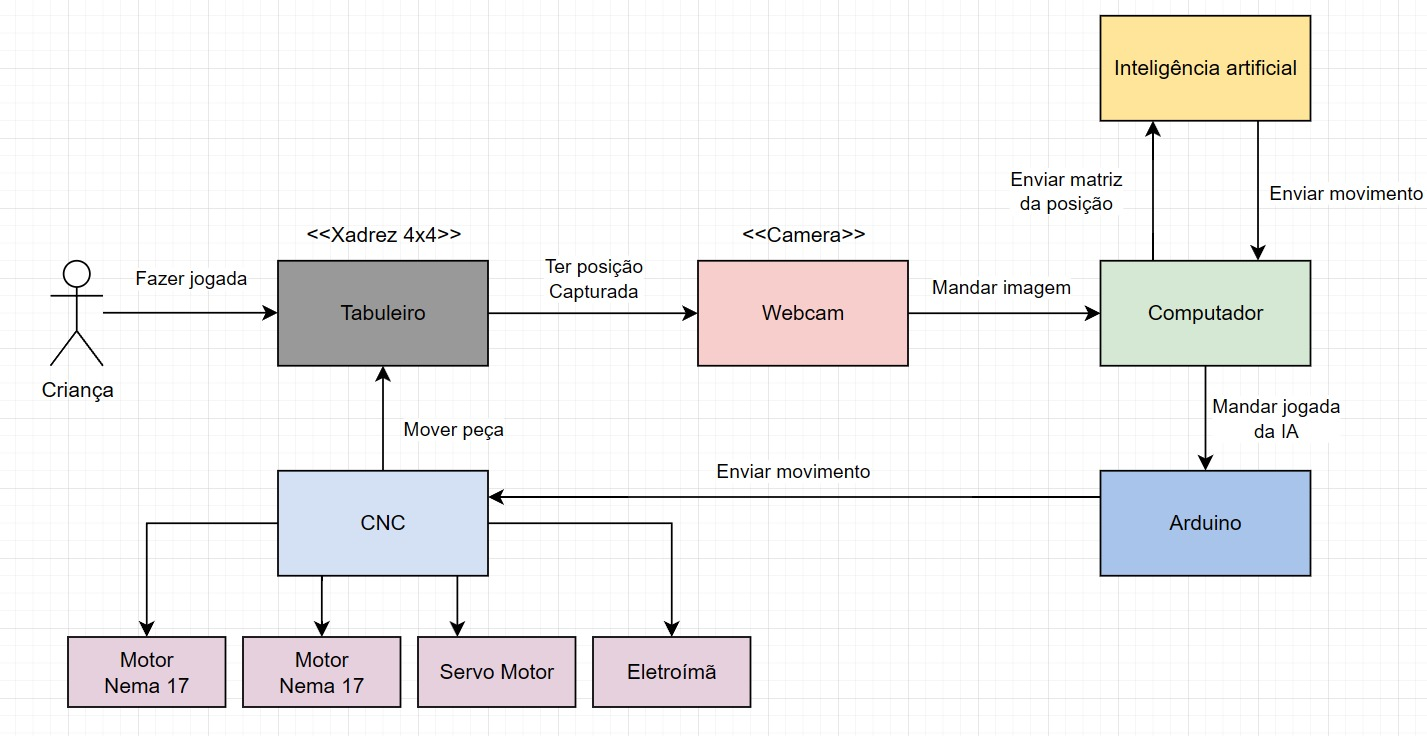
\includegraphics[width=1.0\textwidth]{images/diagrama.jpeg}   
    \caption{Diagrama de Blocos do Sistema Minichess}  
    \label{fig:diagrama}  
\end{figure}  

\begin{figure}[H]  
    \centering  
    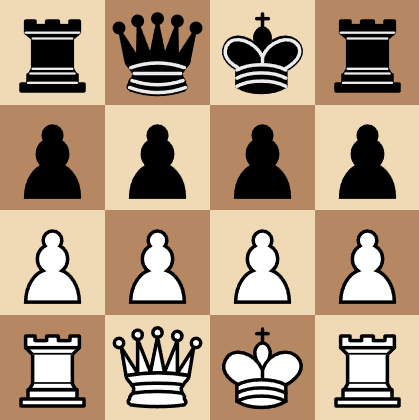
\includegraphics[width=0.5\textwidth]{images/minichess4x4.png}   
    \caption{Tabuleiro do Minichess 4x4}  
    \label{fig:modelo_cnc}  
\end{figure}  

\vspace{1em}  

% --- SEÇÃO: DESCRIÇÃO DO SOFTWARE ---  
\section{Descrição do Software}  
O software deste projeto é responsável por:  
\begin{itemize}  
    \item Implementar a lógica do jogo e a Inteligência Artificial com Machine Learning, utilizando o algoritmo \textbf{Q-learning} (aprendizado por reforço) para tomada de decisão. O agente aprende a otimizar suas jogadas através de um processo iterativo, onde cada ação é associada a um valor que representa a recompensa esperada em longo prazo. O algoritmo equilibra novas jogadas e jogadas anteriores, ajustando-se dinamicamente conforme interage com o jogador. A função de recompensa é definida para priorizar vitórias, evitar derrotas e incentivar movimentos estratégicos no tabuleiro 4x4.  

    \item Capturar e processar imagens do tabuleiro físico utilizando a biblioteca OpenCV. As técnicas incluem detecção de cores, filtragem de bordas e comparação de contornos para identificar a posição das peças. A imagem é recortada para isolar o tabuleiro e evitar interferências externas.  

    \item Gerenciar a comunicação direta entre o computador e o Arduino via protocolo serial, utilizando a biblioteca PySerial para envio de comandos em G-Code. O fluxo é coordenado por um script único que integra a visão computacional, a IA e o controle do CNC, garantindo sincronização entre a decisão da jogada e a movimentação física das peças.  
\end{itemize}  

% --- SEÇÃO: DESCRIÇÃO DO HARDWARE ---  
\section{Descrição do Hardware}  
Para a realização do jogo físico, o sistema conta com os seguintes componentes de hardware:  
\begin{itemize}  
    \item \textbf{Computador com Câmera:} Utilizado para capturar imagens do tabuleiro (resolução 1920x1080) e processar as informações necessárias para a tomada de decisão. A câmera é fixada em uma estrutura de suporte 3D impressa, posicionada verticalmente para garantir visibilidade total do tabuleiro.  
    \item \textbf{Arduino UNO com CNC Shield V3:} Responsável por controlar os motores de passo (Nema 17) e o servo motor SG90. A CNC Shield utiliza drivers A4988 e um relé para acionamento do eletroímã de 12V.  
    \item \textbf{Sistema CNC CoreXY:} Composto por dois motores de passo para movimento no plano XY, seguindo o arranjo CoreXY. O eixo Z é controlado por um servo motor, responsável por abaixar e levantar o eletroímã.  
    \item \textbf{Fonte de Alimentação:} Duas fontes de 12V 5A são utilizadas: uma para os motores de passo e ventoinhas de refrigeração, e outra exclusiva para o eletroímã.  
	\item \textbf{Placa Universal:} Uma Placa Universal será utilizada para a soldagem de componentes eletrônicos auxiliares para a execução do projeto, tais como atuadores e sensores.
\end{itemize}  

% --- FIGURA: MODELO CNC ---  
\begin{figure}[H]  
    \centering  
    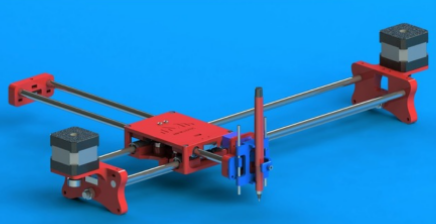
\includegraphics[width=0.5\textwidth]{images/drawingbot.png}   
    \caption{Referência do sistema CNC para movimentação física $^{[5]}$}  
    \label{fig:modelo_cnc}  
\end{figure}  

% --- SEÇÃO: LISTA DE COMPONENTES ---  
\section{Lista de Componentes}  
\begin{itemize}  
    \item \textbf{Software:}  
    \begin{itemize}  
        \item Python 3.8+ (com bibliotecas OpenCV, NumPy e PySerial)  
        \item Firmware GRBL (para interpretação de G-Code no Arduino)  
    \end{itemize}  
    \item \textbf{Hardware:}  
    \begin{itemize}  
        \item Computador com câmera USB Full HD  
        \item Arduino UNO + CNC Shield V3 + Drivers A4988  
        \item 2x Motores de Passo Nema 17 + Correias GT2  
        \item Servo Motor SG90 + Eletroímã 12V  
        \item Fonte de Alimentação 12V 5A (2 unidades)  
        \item Estrutura em MDF cortada a laser + Suportes 3D impressos  
		\item Relé
		\item Placa Universal + sensores e atuadores.
    \end{itemize}  
\end{itemize}  

% --- SEÇÃO: INTEGRAÇÃO ---  
\section{Integração entre Software e Hardware}  
A comunicação entre os módulos é realizada através de um fluxo sequencial unificado:  
\begin{enumerate}  
    \item \textbf{Visão Computacional:} Captura e processamento da imagem do tabuleiro utilizando OpenCV, gerando uma matriz 4x4 que representa o estado atual do jogo.  
    \item \textbf{Inteligência Artificial:} Processamento da matriz pelo algoritmo Q-learning para determinação da melhor jogada, com base em recompensas e aprendizado iterativo.  
    \item \textbf{Controle CNC:} Conversão das coordenadas da jogada em comandos G-Code e envio imediato ao Arduino via comunicação serial, acionando os motores e o eletroímã para movimentação das peças.  
\end{enumerate}  

% --- SEÇÃO: CRONOGRAMA ---  
\section{Cronograma}  

\begin{table}[H]
\centering
\caption{Cronograma}
\label{tab:cronograma}
\renewcommand{\arraystretch}{1.5}
\begin{tabularx}{\textwidth}{Yccc}
\toprule
\rowcolor{marco}
\textbf{Tarefa} & \textbf{Início} & \textbf{Final} & \textbf{Entrega} \\
\midrule

% Marco 1
\rowcolor{marco}
\multicolumn{4}{l}{\textbf{Marco 1}} \\
Elaboração do software com a lógica minichess rodando no computador & 07/04/2025 & 21/04/2025 & - \\
Implementação do algoritmo de Machine Learning & 14/04/2025 & 28/04/2025 & - \\
Fazer os modelos 3D das peças de xadrez planificadas & 14/04/2025 & 28/04/2025 & - \\
Fazer projeto elétrico & 14/04/2025 & 05/05/2025 & - \\
MARCO 1 & - & - & 12/05/2025 \\

% Marco 2
\rowcolor{marco}
\multicolumn{4}{l}{\textbf{Marco 2}} \\
Impressão 3D das peças & 05/05/2025 & 19/05/2025 & - \\
Implementação do algoritmo de reconhecimento das peças & 28/04/2025 & 12/05/2025 & - \\
Construção do tabuleiro 4x4 & 28/04/2025 & 12/05/2025 & - \\
Instalação de suporte para webcam & 05/05/2025 & 19/05/2025 & - \\
MARCO 2 & - & - & 26/05/2025 \\

% Marco 3
\rowcolor{marco}
\multicolumn{4}{l}{\textbf{Marco 3}} \\
Montagem da CNC e de suas respectivas peças & 14/04/2025 & 02/06/2025 & - \\
Calibração do passo da CNC & 12/05/2025 & 02/06/2025 & - \\
Comunicação serial computador - Arduino com CNC & 19/05/2025 & 02/06/2025 & - \\
Soldagem dos componentes eletrônicos em uma placa universal & 19/05/2025 & 02/06/2025 & - \\
MARCO 3 & - & - & 09/06/2025 \\

\bottomrule
\end{tabularx}

\end{table}

\vspace{1em}  

\begin{figure}[H]  
    \centering  
    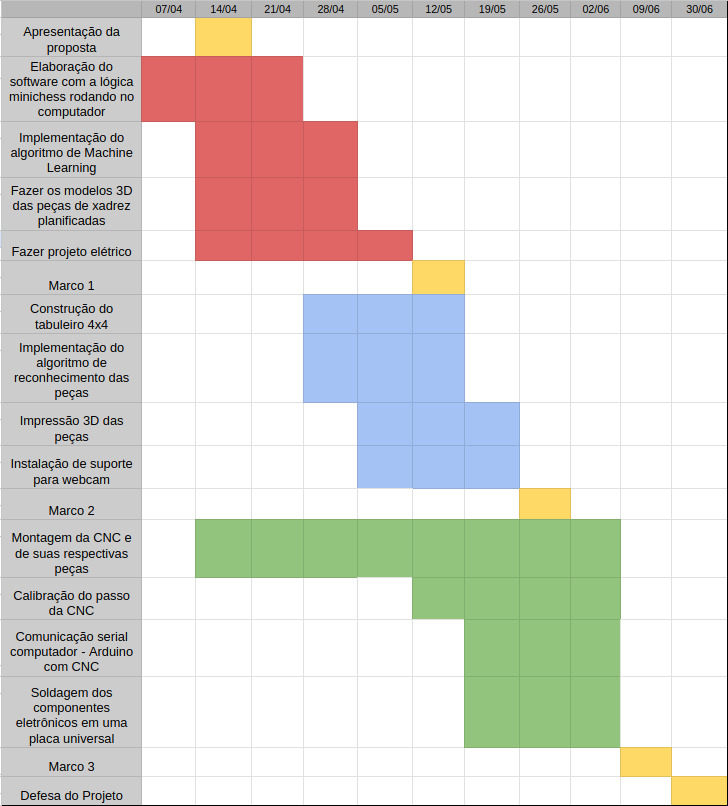
\includegraphics[width=1\textwidth]{images/cronograma2.jpg}   
    \caption{Diagrama de Gantt}  
    \label{fig:cronograma_projeto}  
\end{figure}  

\vspace{1em}  

% --- REFERÊNCIAS ---  
\begin{thebibliography}{9}  
\bibitem{ref1} \href{https://arxiv.org/abs/2109.11434}{https://arxiv.org/abs/2109.11434}  
\bibitem{ref2} \href{https://arxiv.org/abs/2106.11034}{https://arxiv.org/abs/2106.11034}  
\bibitem{ref3} \href{https://journals.copmadrid.org/psed/art/psed2025a10}{https://journals.copmadrid.org/psed/art/psed2025a10}  
\bibitem{ref4} \href{https://pubmed.ncbi.nlm.nih.gov/28494023/}{https://pubmed.ncbi.nlm.nih.gov/28494023/}  
\bibitem{ref5} MakerC. \textit{DrawingBot: Open Source Plotter}. Thingiverse, 2016. Disponível em: \url{https://www.thingiverse.com/thing:1517211}.  
\bibitem{ref6} \url{https://ieeexplore.ieee.org/document/10179542}
\bibitem{ref7} Conrado, A. \textit{Controle de Máquinas CNC com GRBL}. Revista de Engenharia, 2017.  
\bibitem{ref8} Handson Technology. \textit{CNC Shield V3 Documentation}. 2021. Disponível em: \url{https://www.handsontec.com}.  
\end{thebibliography}  

\end{document}  
